\documentclass[a4paper]{book}
% chktex-file 
% chktex-file 3
\usepackage{geometry}
% make full use of A4 papers
\geometry{margin=1.5cm, vmargin={0pt,1cm}}
\setlength{\topmargin}{-1cm}
\setlength{\paperheight}{29.7cm}
\setlength{\textheight}{25.1cm}

% auto adjust the marginals
\usepackage{marginfix}

\usepackage{amsfonts}
\usepackage{amsmath}
\usepackage{amssymb}
\usepackage{amsthm}
% \usepackage{CJKutf8}   % for Chinese characters
\usepackage{ctex}
\usepackage{enumerate}
\usepackage{graphicx}  % for figures
\usepackage{layout}
\usepackage{multicol}  % multiple columns to reduce number of pages
\usepackage{mathrsfs}
\usepackage{fancyhdr}
\usepackage{subfigure}
\usepackage{tcolorbox}
\usepackage{tikz-cd}
\usepackage{listings}
\usepackage{xcolor} %代码高亮
\usepackage{braket}
\usepackage{graphicx}
\usepackage{subfigure}
% ------------------
% common commands %
% ------------------
% differentiation
\newcommand{\gen}[1]{\left\langle#1 \right\rangle}
\newcommand{\dif}{\mathrm{d}}
\newcommand{\difPx}[1]{\frac{\partial#1}{\partial x}}
\newcommand{\difPy}[1]{\frac{\partial#1}{\partial y}}
\newcommand{\Dim}{\mathrm{D}}
\newcommand{\avg}[1]{\left\langle#1 \right\rangle}
\newcommand{\sgn}{\mathrm{sgn}}
\newcommand{\Span}{\mathrm{span}}
\newcommand{\dom}{\mathrm{dom}}
\newcommand{\Arity}{\mathrm{arity}}
\newcommand{\Int}{\mathrm{Int}}
\newcommand{\Ext}{\mathrm{Ext}}
\newcommand{\Cl}{\mathrm{Cl}}
\newcommand{\Fr}{\mathrm{Fr}}
% group is generated by
\newcommand{\grb}[1]{\left\langle#1 \right\rangle}
% rank
\newcommand{\rank}{\mathrm{rank}}
\newcommand{\Iden}{\mathrm{Id}}

% this environment is for solutions of examples and exercises
\newenvironment{solution}%
{\noindent\textbf{Solution.}}%
{\qedhere}
% the following command is for disabling environments
% so that their contents do not show up in the pdf.
\makeatletter
\newcommand{\voidenvironment}[1]{%
  \expandafter\providecommand\csname env@#1@save@env\endcsname{}%
  \expandafter\providecommand\csname env@#1@process\endcsname{}%
  \@ifundefined{#1}{}{\RenewEnviron{#1}{}}%
}
\makeatother

% ---------------------------------------------
% commands specifically for complex analysis %
% ---------------------------------------------
% complex conjugate
\newcommand{\ccg}[1]{\overline{#1}}
% the imaginary unit
\newcommand{\ii}{\mathbf{i}}
% \newcommand{\ii}{\boldsymbol{i}}
% the real part
\newcommand{\Rez}{\mathrm{Re}\,}
% the imaginary part
\newcommand{\Imz}{\mathrm{Im}\,}
% punctured complex plane
\newcommand{\pcp}{\mathbb{C}^{\bullet}}
% the principle branch of the logarithm
\newcommand{\Log}{\mathrm{Log}}
% the principle value of a nonzero complex number
\newcommand{\Arg}{\mathrm{Arg}}
\newcommand{\Null}{\mathrm{null}}
\newcommand{\Range}{\mathrm{range}}
\newcommand{\Ker}{\mathrm{ker}}
\newcommand{\Iso}{\mathrm{Iso}}
\newcommand{\Aut}{\mathrm{Aut}}
\newcommand{\ord}{\mathrm{ord}}
\newcommand{\Res}{\mathrm{Res}}
% \newcommand{\GL2R}{\mathrm{GL}(2,\mathbb{R})}
\newcommand{\GL}{\mathrm{GL}}
\newcommand{\SL}{\mathrm{SL}}
\newcommand{\Dist}[2]{\left|{#1}-{#2}\right|}

\newcommand\tbbint{{-\mkern-16mu\int}}
\newcommand\tbint{{\mathchar'26 -\mkern-14mu\int}}
\newcommand\dbbint{{-\mkern-20mu\int}}
\newcommand\dbint{{\mathchar'26 -\mkern-26mu\int}}
\newcommand\bint{
  {\mathchoice{\dbint}{\tbint}{\tbint}{\tbint}}
}
\newcommand\bbint{
  {\mathchoice{\dbbint}{\tbbint}{\tbbint}{\tbbint}}
}





% ----------------------------------------
% theorem and theorem-like environments %
% ----------------------------------------
\numberwithin{equation}{chapter}
\theoremstyle{definition}

\newtheorem{thm}{Theorem}[chapter]
\newtheorem{axm}[thm]{Axiom}
\newtheorem{alg}[thm]{Algorithm}
\newtheorem{asm}[thm]{Assumption}
\newtheorem{defn}[thm]{Definition}
\newtheorem{prop}[thm]{Proposition}
\newtheorem{rul}[thm]{Rule}
\newtheorem{coro}[thm]{Corollary}
\newtheorem{lem}[thm]{Lemma}
\newtheorem{exm}{Example}[chapter]
\newtheorem{rem}{Remark}[chapter]
\newtheorem{exc}[exm]{Exercise}
\newtheorem{frm}[thm]{Formula}
\newtheorem{ntn}{Notation}

% for complying with the convention in the textbook
\newtheorem{rmk}[thm]{Remark}


% \lstset{
%	backgroundcolor=\color{red!50!green!50!blue!50},%代码块背景色为浅灰色
%	rulesepcolor= \color{gray}, %代码块边框颜色
%	breaklines=true,  %代码过长则换行
%	numbers=left, %行号在左侧显示
%	numberstyle= \small,%行号字体
%	keywordstyle= \color{blue},%关键字颜色
%	commentstyle=\color{gray}, %注释颜色
%	frame=shadowbox%用方框框住代码块
% }
\lstset{
  columns=fixed,
  numbers=left,                                        % 在左侧显示行号
  numberstyle=\tiny\color{gray},                       % 设定行号格式
  frame=none,                                          % 不显示背景边框
  backgroundcolor=\color[RGB]{245,245,244},            % 设定背景颜色
  keywordstyle=\color[RGB]{40,40,255},                 % 设定关键字颜色
  numberstyle=\footnotesize\color{darkgray},
  commentstyle=\it\color[RGB]{0,96,96},                % 设置代码注释的格式
  stringstyle=\rmfamily\slshape\color[RGB]{128,0,0},   % 设置字符串格式
  showstringspaces=false,                              % 不显示字符串中的空格
  language=c++,                                        % 设置语言
}

% ----------------------
% the end of preamble %
% ----------------------

\begin{document}
\pagestyle{empty}
\pagenumbering{roman}
% 
% \tableofcontents
% \clearpage

% \pagestyle{fancy}
% \fancyhead{}
% \lhead{Qinghai Zhang}
% \chead{Notes on Algebraic Topology}
% \rhead{Fall 2018}


\setcounter{chapter}{0}
\pagenumbering{arabic}
% \setcounter{page}{0}

% --------------------------------------------------------
% uncomment the following to remove these environments
% to generate handouts for students.
% --------------------------------------------------------
% \begingroup
% \voidenvironment{rem}%
% \voidenvironment{proof}%
% \voidenvironment{solution}%


% each chapter is factored into a separate file.

\chapter{Homework 12235005 谭焱}

\section{Program1}
\input{sec/Program1}

\section{BDF method stability domain}
\exc Try to display the stability domain 
for the BDF methods for $3\leq p \leq 6$.

\begin{solution}
\begin{itemize}
  \item $p = 3$. the characteristic equation is 
  \[(1 - \frac{6}{11} \mu) z^3 - \frac{18}{11} z ^2 
   + \frac{9}{11} z - \frac{2}{11} = 0. \]

   \item $p = 4$. the characteristic equation is 
  \[(1 - \frac{12}{25} \mu) z^4 - \frac{48}{25} z ^3 
   + \frac{36}{25} z^2 - \frac{16}{25} z 
   + \frac{3}{25} = 0. \]

   \item $p = 5$. the characteristic equation is 
   \[(1 - \frac{60}{137} \mu) z^5 - \frac{300}{137} z ^4 
   + \frac{300}{137} z^3 - \frac{200}{137} z^2 
   + \frac{75}{137} z - \frac{12}{137} = 0. \]

   \item $p = 6$. the characteristic equation is 
   \[(1 - \frac{60}{147} \mu) z^6 - \frac{360}{147} z ^5 
  + \frac{450}{147} z^4 - \frac{400}{147} z^3 
  + \frac{225}{147} z^2 - \frac{72}{147} z 
  + \frac{10}{147} = 0. \]
\end{itemize}

don't know how to plot, only find wiki picture;
\begin{figure}[!h]
  \caption{}
  \centering
  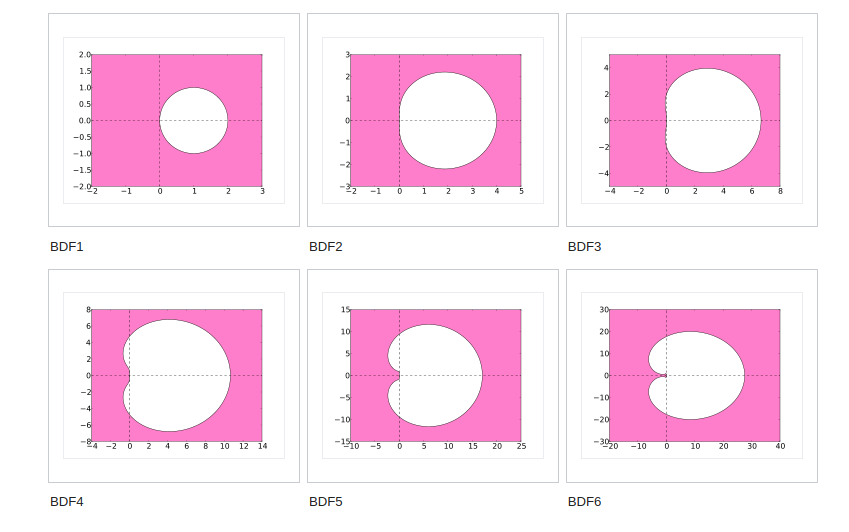
\includegraphics[height=3in]{fig/stabilityDomain.png}
  %\caption{fig1}
 
\end{figure}
\end{solution}



\section{2.2.1}
\exc Derive the stability condition 
for Simpson’s rule (2.2.10) when used for
the equation $u_t = u_x$ with $Q_4$ .

\begin{solution}
 the characteristic equation is 
  \[(1 - \frac{\mu}{3}) z^2 - \frac{4 \mu}{3} z 
    - (1 + \frac{\mu}{3}) = 0. \]
    with two roots be 
    \[|z_{1, 2}| = |\frac{2\mu \pm \sqrt{3\mu^2 + 9}}
    {3 - \mu}| \leq 1 .\]
    have $|2\mu + \sqrt{3\mu^2 + 9}| \leq |3 - \mu|$ 
    and $ |2\mu - \sqrt{3\mu^2 + 9}| \leq |3 - \mu|$ get 
    $Re\ \mu = 0$, and $|Im\ \mu| \leq \sqrt{3}$.

    By $Q_4 = i \lambda \sin(\xi)(1 - \frac{2}{3} \sin^2 
    \frac{\xi}{2})$, induce 
    \[|\lambda \sin(\xi) (\frac{2}{3} - \frac{1}{3}
    \cos \xi)| \leq \sqrt{3}.\]

    Solve it $ \frac{k}{h} = \lambda \leq
     \sqrt[4]{27}(\sqrt{6} - \sqrt{2})$
    

\end{solution}

\end{document}